\documentclass[a4paper, 11pt]{article}
\usepackage{graphicx}
\usepackage{multicol}
\usepackage{tabularx}
\usepackage{enumitem}
\usepackage[a4paper, margin=1.8cm]{geometry}
\usepackage{listings}
\usepackage{amssymb}
\usepackage{gvv}
\usepackage{gvv-book}
\usepackage{amsmath}
\usepackage{setspace}
\usepackage{caption}
\usepackage{tfrupee}
\usepackage{float}

\graphicspath{ {./figs} }

\begin{document}
\begin{center}
    \huge{CS: COMPUTER SCIENCE AND INFORMATION TECHNOLOGY-2024, SET-1}\\
    \large{EE25BTECH11041 - Naman Kumar}
\end{center}


\begin{enumerate}
    \item If $\rightarrow$ denotes increasing order of intensity, then the meaning of the words [dry $\rightarrow$ arid $\rightarrow$ parched] is analogous to [diet $\rightarrow$ fast $\rightarrow$ \underline{\hspace{2cm}}].\\Which one of the given options is appropriate to fill the blank?
    \begin{enumerate}
    \begin{multicols}{4}
        \item starve
        \item reject
        \item feast
        \item deny
    \end{multicols}
    \end{enumerate}
    \hfill{\brak{\text{GATE CS 2024}}}
    
    \item If two distinct non-zero real variables $x$ and $y$ are such that \brak{x+y} is proportional to \brak{x-y}, then the value of $\frac{x}{y}$
    \begin{enumerate}
    \begin{multicols}{2}
        \item depends on $xy$
        \item depends only on $x$ and not on $y$
        \item depends only on $y$ and not on $x$
        \item is a constant
    \end{multicols}
    \end{enumerate}
    \hfill{\brak{\text{GATE CS 2024}}}
    
    \item Consider the following sample of numbers:
    
    $9, 18, 11, 14, 15, 17, 10, 69, 11, 13$
    
    The median of the sample is
    \begin{enumerate}
    \begin{multicols}{4}
        \item $13.5$
        \item $14$
        \item $11$
        \item $18.7$
    \end{multicols}
    \end{enumerate}
    \hfill{\brak{\text{GATE CS 2024}}}
    
    \item The number of coins of \rupee$1$, \rupee$5$, and \rupee$10$ denominations that a person has are in the ratio $5 \colon 3 \colon 13$. Of the total amount, the percentage of money in ₹$5$ coins is
    \begin{enumerate}
    \begin{multicols}{4}
        \item $14\frac{2}{7}\%$
        \item $25\%$
        \item $10\%$
        \item $15\%$
    \end{multicols}
    \end{enumerate}
    \hfill{\brak{\text{GATE CS 2024}}}
    
    \item For positive non-zero real variables $p$ and $q$, if
    \begin{center}
    $\log\brak{p^{2}+q^{2}}=\log p+\log q+2 \log 3$,
    \end{center}
    then, the value of $\frac{p^{4}+q^{4}}{p^{2}q^{2}}$ is
    \begin{enumerate}
    \begin{multicols}{4}
        \item $79$
        \item $81$
        \item $9$
        \item $83$
    \end{multicols}
    \end{enumerate}
    
    \hfill{\brak{\text{GATE CS 2024}}}
    \item In the given text, the blanks are numbered \brak{i}-\brak{iv}. Select the best match for all the blanks.
    
    Steve was advised to keep his head \underline{\hspace{1cm}}\brak{i}\underline{\hspace{1cm}} before heading \underline{\hspace{1cm}}\brak{ii}\underline{\hspace{1cm}} to bat; for, while he had a head \underline{\hspace{1cm}}\brak{iii}\underline{\hspace{1cm}} his shoulders, batting, he could only do so with a cool head \underline{\hspace{1cm}}\brak{iv}\underline{\hspace{1cm}}.

    \begin{enumerate}
        \item \brak{i} down \quad \brak{ii} down \quad \brak{iii} on \quad \brak{iv} for
        \item \brak{i} on \quad \brak{ii} down \quad \brak{iii} for \quad \brak{iv} on
        \item \brak{i} down \quad \brak{ii} out \quad \brak{iii} on \quad \brak{iv} for
        \item \brak{i} on \quad \brak{ii} out \quad \brak{iii} for \quad \brak{iv} on
    \end{enumerate}
    \newpage
    \hfill{\brak{\text{GATE CS 2024}}}
    
    \item A rectangular paper sheet of dimensions $54$ cm x $4$ cm is taken. The two longer edges of the sheet are joined together to create a cylindrical tube. A cube whose surface area is equal to the area of the sheet is also taken.\\
    Then, the ratio of the volume of the cylindrical tube to the volume of the cube is
    \begin{enumerate}
    \begin{multicols}{4}
        \item $1/\pi$
        \item $2/\pi$
        \item $3/\pi$
        \item $4/\pi$
    \end{multicols}
    \end{enumerate}
    \hfill{\brak{\text{GATE CS 2024}}}
    
    \item The pie chart presents the percentage contribution of different macronutrients to a typical $2,000$ kcal diet of a person.
    
    \begin{figure}[H]
        \centering
        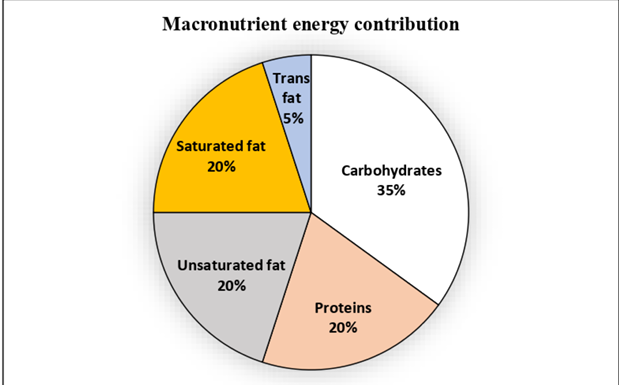
\includegraphics[width=0.6\columnwidth]{q8}
        \caption*{}
        \label{fig:q8}
    \end{figure}
    
    The typical energy density \brak{kcal/g} of these macronutrients is given in the table.
    
    \begin{table}[H]
        \centering
        \begin{tabular}{|l|c|}
        \hline
        \textbf{Macronutrient} & \textbf{Energy density \brak{kcal/g}} \\
        \hline
        Carbohydrates & $4$ \\
        \hline
        Proteins & $4$ \\
        \hline
        Unsaturated fat & $9$ \\
        \hline
        Saturated fat & $9$ \\
        \hline
        Trans fat & $9$ \\
        \hline
        \end{tabular}
        \caption*{}
        \label{tab:q8}
    \end{table}
    
    The total fat \brak{all three types}, in grams, this person consumes is
    \begin{enumerate}
    \begin{multicols}{4}
        \item $44.4$
        \item $77.8$
        \item $100$
        \item $3,600$
    \end{multicols}
    \end{enumerate}

    \hfill{\brak{\text{GATE CS 2024}}}
    \item A rectangular paper of $20 \text{ cm} \times 8 \text{ cm}$ is folded 3 times. Each fold is made along the line of symmetry, which is perpendicular to its long edge. The perimeter of the final folded sheet \brak{in cm} is
    \begin{enumerate}
        \begin{multicols}{4}
            \item $18$
            \item $24$
            \item $20$
            \item $21$
        \end{multicols}
    \end{enumerate}
    \hfill{\brak{\text{GATE CS 2024}}}

    \item The least number of squares to be added in the figure to make AB a line of symmetry is
    
    \begin{figure}[H]
        \centering
        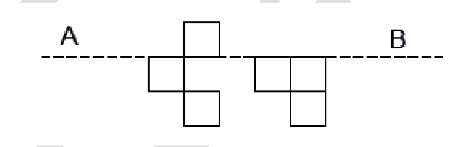
\includegraphics[width=\columnwidth]{figs/q10.png}
        \caption*{}
        \label{fig:q10}
    \end{figure}
    \begin{enumerate}
        \begin{multicols}{4}
            \item $6$
            \item $4$
            \item $5$
            \item $7$
        \end{multicols}
    \end{enumerate}
    \hfill{\brak{\text{GATE CS 2024}}}

    \item Let $f \colon \mathbb{R} \rightarrow \mathbb{R}$ be a function such that $f(x) = \max\{x, x^3\}$ for $x \in \mathbb{R}$, where $\mathbb{R}$ is the set of all real numbers. The set of all points where $f(x)$ is NOT differentiable is
    \begin{enumerate}
        \begin{multicols}{2}
            \item $\{-1, 1, 2\}$
            \item $\{-2, -1, 1\}$
            \item $\{0, 1\}$
            \item $\{-1, 0, 1\}$
        \end{multicols}
    \end{enumerate}
    \hfill{\brak{\text{GATE CS 2024}}}

    \item The product of all eigenvalues of the matrix $\myvec{1 & 2 & 3 \\ 4 & 5 & 6 \\ 7 & 8 & 9}$ is
    \begin{enumerate}
        \begin{multicols}{4}
            \item $0$
            \item $-1$
            \item $1$
            \item $2$
        \end{multicols}
    \end{enumerate}
    \hfill{\brak{\text{GATE CS 2024}}}

    \item Consider a system that uses $5$ bits for representing signed integers in 2's complement format. In this system, two integers A and B are represented as $A=01010$ and $B=11010$. Which one of the following operations will result in either an arithmetic overflow or an arithmetic underflow?
    \begin{enumerate}
        \begin{multicols}{2}
            \item $A+B$
            \item $A-B$
            \item $B-A$
            \item $2*B$
        \end{multicols}
    \end{enumerate}

    \hfill{\brak{\text{GATE CS 2024}}}
    \item Consider a permutation sampled uniformly at random from the set of all permutations of $\{1, 2, 3, \dots, n\}$ for some $n \ge 4$. Let X be the event that $1$ occurs before $2$ in the permutation, and Y the event that $3$ occurs before $4$. Which one of the following statements is TRUE?

    \begin{enumerate}
        \item The events X and Y are mutually exclusive
        \item The events X and Y are independent
        \item Either event X or Y must occur
        \item Event X is more likely than event Y
    \end{enumerate}

    \hfill{\brak{\text{GATE CS 2024}}}
    \item Which one of the following statements is FALSE?

    \begin{enumerate}
        \item In the cycle stealing mode of DMA, one word of data is transferred between an I/O device and main memory in a stolen cycle
        \item For bulk data transfer, the burst mode of DMA has a higher throughput than the cycle stealing mode
        \item Programmed I/O mechanism has a better CPU utilization than the interrupt driven I/O mechanism
        \item The CPU can start executing an interrupt service routine faster with vectored interrupts than with non-vectored interrupts
    \end{enumerate}
    \hfill{\brak{\text{GATE CS 2024}}}

    \item A user starts browsing a webpage hosted at a remote server. The browser opens a single TCP connection to fetch the entire webpage from the server. The webpage consists of a top-level index page with multiple embedded image objects. Assume that all caches \brak{e.g., DNS cache, browser cache} are all initially empty. The following packets leave the user's computer in some order.
    
    \begin{enumerate}[label=(\roman*)]
        \item HTTP GET request for the index page
        \item DNS request to resolve the web server's name to its IP address
        \item HTTP GET request for an image object
        \item TCP SYN to open a connection to the web server
    \end{enumerate}
    
    Which one of the following is the CORRECT chronological order \brak{earliest in time to latest} of the packets leaving the computer?

    \begin{enumerate}
        \item \brak{iv}, \brak{ii}, \brak{iii}, \brak{i}
        \item \brak{ii}, \brak{iv}, \brak{iii}, \brak{i}
        \item \brak{ii}, \brak{iv}, \brak{i}, \brak{iii}
        \item \brak{iv}, \brak{ii}, \brak{i}, \brak{iii}
    \end{enumerate}
    \hfill{\brak{\text{GATE CS 2024}}}

    \item Given an array of size $N$, we want to check if the array is sorted \brak{in either ascending or descending order}. An algorithm solves this problem by making a single pass through the array and comparing each element of the array only with its immediate successor. The worst-case time complexity of this algorithm is

    \begin{enumerate}
        \item both $O(N)$ and $\Omega(N)$
        \item $O(N)$ but not $\Omega(N)$
        \item $\Omega(N)$ but not $O(N)$
        \item neither $O(N)$ nor $\Omega(N)$
    \end{enumerate}
    \hfill{\brak{\text{GATE CS 2024}}}

    \item Consider the following C program:
    \begin{lstlisting}[language=C]
#include <stdio.h>

int main() {
    int a = 6;
    int b = 0;
    while (a < 10) {
        a = a / 12 + 1;
        a += b;
    }
    printf("%d", a);
    return 0;
}
    \end{lstlisting}
    Which one of the following statements is CORRECT?

    \begin{enumerate}
        \item The program prints 9 as output
        \item The program prints 10 as output
        \item The program gets stuck in an infinite loop
        \item The program prints 6 as output
    \end{enumerate}
    \hfill{\brak{\text{GATE CS 2024}}}

    \item Consider the following C program:\\
    \begin{minipage}{5cm}
    \begin{lstlisting}       
    #include <stdio.h>
    
    void fx()
    int main() {
        fX();
        return 0;
    }
    
    \end{lstlisting}
    \end{minipage}
    \begin{minipage}{5cm}
    \begin{lstlisting}   
    void fx() {
    char a;
    if ((a = getchar()) != '\n') 
        fX();
    
    if (a != '\n')
        putchar(a);
    
    \end{lstlisting}
    \end{minipage}\\
    Assume that the input to the program from the command line is 1234 followed by a newline character. Which one of the following statements is CORRECT? 
    \begin{enumerate}
        \begin{multicols}{2}
        \item The program will not terminate
        \item The program will terminate with no output 
        \item The program will terminate with 4321 as output 
        \item The program will terminate with 1234 as output
        \end{multicols}
    \end{enumerate}
    \hfill{\brak{\text{GATE CS 2024}}}

    \item Let S be the specification: "Instructors teach courses. Students register for courses. Courses are allocated classrooms. Instructors guide students." Which one of the following ER diagrams CORRECTLY represents S?

    \begin{figure}[H]
        \centering
        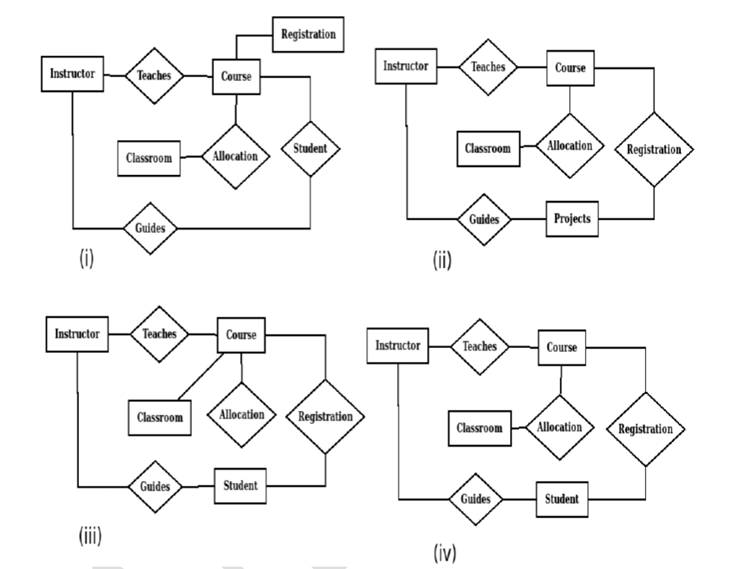
\includegraphics[width=0.7\columnwidth]{figs/q20.png}       
        \label{fig:placeholder}
    \end{figure}
    \begin{enumerate}
        \begin{multicols}{4}
        \item \brak{i}
        \item \brak{ii}
        \item \brak{iii}
        \item \brak{iv}
        \end{multicols}
    \end{enumerate}

   \hfill{\brak{\text{GATE CS 2024}}}
    \item In a B+ tree, the requirement of at least half-full \brak{50\%} node occupancy is relaxed for which one of the following cases?

    \begin{enumerate}
        \item Only the root node
        \item All leaf nodes
        \item All internal nodes
        \item Only the leftmost leaf node
    \end{enumerate}
    \hfill{\brak{\text{GATE CS 2024}}}

    \item Which of the following statements about a relation R in first normal form \brak{1NF} is/are TRUE?

    \begin{enumerate}
        \item R can have a multi-attribute key
        \item R cannot have a foreign key
        \item R cannot have a composite attribute
        \item R cannot have more than one candidate key
    \end{enumerate}
    \hfill{\brak{\text{GATE CS 2024}}}

    \item Let $L_1$, $L_2$ be two regular languages and $L_3$ a language which is not regular. Which of the following statements is/are always TRUE?

    \begin{enumerate}
        \item $L_1 = L_2$ if and only if $L_1 \cap \overline{L_2} = \phi$
        \item $L_1 \cup L_3$ is not regular
        \item $\overline{L_3}$ is not regular
        \item $\overline{L_1} \cup \overline{L_2}$ is regular
    \end{enumerate}
    \hfill{\brak{\text{GATE CS 2024}}}

    \item Which of the following statements about threads is/are TRUE?

    \begin{enumerate}
        \item Threads can only be implemented in kernel space
        \item Each thread has its own file descriptor table for open files
        \item All the threads belonging to a process share a common stack
        \item Threads belonging to a process are by default not protected from each other
    \end{enumerate}
    \hfill{\brak{\text{GATE CS 2024}}}

    \item Which of the following process state transitions is/are NOT possible?
    \begin{enumerate}
        \item Running to Ready
        \item Waiting to Running
        \item Ready to Waiting
        \item Running to Terminated
    \end{enumerate}
    \hfill{\brak{\text{GATE CS 2024}}}

    \item Which of the following is/are Bottom-Up Parser\brak{s}?
    \begin{enumerate}
        \item Shift-reduce Parser
        \item Predictive Parser
        \item $LL(1)$ Parser
        \item LR Parser
    \end{enumerate}
    \hfill{\brak{\text{GATE CS 2024}}}

    \item Let A and B be two events in a probability space with $P(A) = 0.3$, $P(B) = 0.5$, and $P(A \cap B) = 0.1$. Which of the following statements is/are TRUE?
    \begin{enumerate}
        \item The two events A and B are independent
        \item $P(A \cup B) = 0.7$
        \item $P(A \cap B^c) = 0.2$, where $B^c$ is the complement of the event B
        \item $P(A^c \cap B^c) = 0.4$ where $A^c$ and $B^c$ are the complements of the events A and B, respectively
    \end{enumerate}
    \hfill{\brak{\text{GATE CS 2024}}}

    \item Consider the circuit shown below where the gates may have propagation delays. Assume that all signal transitions occur instantaneously and that wires have no delays. Which of the following statements about the circuit is/are CORRECT?

    \begin{figure}[H]
        \centering
        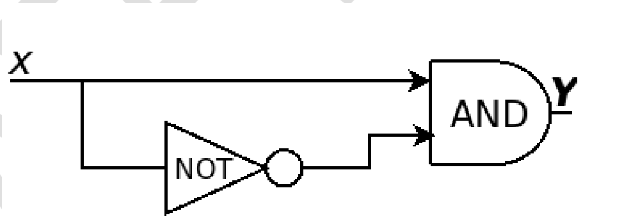
\includegraphics[width=0.5\columnwidth]{figs/q28.png}
        \caption*{}
        \label{fig:q28}
    \end{figure}

    \begin{enumerate}
        \item With no propagation delays, the output Y is always logic Zero
        \item With no propagation delays, the output Y is always logic One
        \item With propagation delays, the output Y can have a transient logic One after X transitions from logic Zero to logic One
        \item With propagation delays, the output Y can have a transient logic Zero after X transitions from logic One to logic Zero
    \end{enumerate}
    \hfill{\brak{\text{GATE CS 2024}}}

    \item TCP client P successfully establishes a connection to TCP server Q. Let $N_P$ denote the sequence number in the SYN sent from P to Q. Let $N_Q$ denote the acknowledgement number in the SYN ACK from Q to P. Which of the following statements is/are CORRECT?
    \begin{enumerate}
        \item The sequence number $N_P$ is chosen randomly by P
        \item The sequence number $N_P$ is always 0 for a new connection
        \item The acknowledgement number $N_Q$ is equal to $N_P$
        \item The acknowledgement number $N_Q$ is $N_P + 1$
    \end{enumerate}
    \hfill{\brak{\text{GATE CS 2024}}}

    \item Consider a 5-stage pipelined processor with Instruction Fetch \brak{IF}, Instruction Decode \brak{ID}, Execute \brak{EX}, Memory Access \brak{MEM}, and Register Writeback \brak{WB} stages. Which of the following statements about forwarding is/are CORRECT?
    \begin{enumerate}
        \item Forwarding means the result from a source stage of an instruction is passed to the destination stage of a later instruction
        \item In forwarding, data from the output of the MEM stage can be passed on to the input of the EX stage of the next instruction
        \item Forwarding cannot prevent all pipeline stalls
        \item Forwarding does not require any extra hardware to retrieve the data from the pipeline stages
    \end{enumerate}
    \hfill{\brak{\text{GATE CS 2024}}}

    \item Which of the following fields is/are modified in the IP header of a packet going out of a network address translation \brak{NAT} device from an internal network to an external network?
    \begin{enumerate}
        \item Source IP
        \item Destination IP
        \item Header Checksum
        \item Total Length
    \end{enumerate}
    \hfill{\brak{\text{GATE CS 2024}}}

    \item Let A and B be non-empty finite sets such that there exist one-to-one and onto functions \brak{i} from A to B and \brak{ii} from $A \times A$ to $A \cup B$. The number of possible values of $|A|$ is \underline{\hspace{2cm}}.
    \item Consider the operator precedence and associativity rules for the integer arithmetic operators given in the table below.
    
    \begin{table}[H]
        \centering
        \begin{tabular}{|c|l|l|}
        \hline
        \textbf{Operator} & \textbf{Precedence} & \textbf{Associativity} \\
        \hline
        + & Highest & Left \\
        \hline
        - & High & Right \\
        \hline
        * & Medium & Right \\
        \hline
        / & Low & Right \\
        \hline
        \end{tabular}
        \caption*{}
        \label{tab:q33}
    \end{table}
    
    The value of the expression $3+1+5*2/7+2-4-7-6/2$ as per the above rules is \underline{\hspace{2cm}}.
    \hfill{\brak{\text{GATE CS 2024}}}

    \item The number of spanning trees in a complete graph of 4 vertices labelled A, B, C, and D is \underline{\hspace{2cm}}.

    \hfill{\brak{\text{GATE CS 2024}}}

    \item Consider the following two relations, $R(A,B)$ and $S(A,C)$:
    
    \begin{minipage}{0.45\textwidth}
        \centering
        \begin{tabular}{|c|c|}
            \hline
            \multicolumn{2}{|c|}{\textbf{R}} \\
            \hline
            \textbf{A} & \textbf{B} \\
            \hline
            10 & 20 \\
            \hline
            20 & 30 \\
            \hline
            30 & 40 \\
            \hline
            30 & 50 \\
            \hline
            50 & 95 \\
            \hline
        \end{tabular}
    \end{minipage}
    \begin{minipage}{0.45\textwidth}
        \centering
        \begin{tabular}{|c|c|}
            \hline
            \multicolumn{2}{|c|}{\textbf{S}} \\
            \hline
            \textbf{A} & \textbf{C} \\
            \hline
            10 & 90 \\
            \hline
            30 & 45 \\
            \hline
            40 & 80 \\
            \hline
        \end{tabular}
    \end{minipage}
    
    The total number of tuples in $\sigma_{B<C}(R \bowtie_{R.A=S.A} S)$ is \underline{\hspace{2cm}}.

    \hfill{\brak{\text{GATE CS 2024}}}

    \item Consider a network path P-Q-R between nodes P and R via router Q. Node P sends a file of size $10^6$ bytes to R via this path by splitting the file into chunks of $10^3$ bytes each. Node P sends these chunks one after the other without any wait time between the successive chunk transmissions. Assume that the size of extra headers added to these chunks is negligible, and that the chunk size is less than the MTU.
    
    Each of the links P-Q and Q-R has a bandwidth of $10^6$ bits/sec, and negligible propagation latency. Router Q immediately transmits every packet it receives from P to R, with negligible processing and queueing delays. Router Q can simultaneously receive on link P-Q and transmit on link Q-R.
    
    Assume P starts transmitting the chunks at time $t=0$.
    
    Which one of the following options gives the time \brak{\text{in seconds, rounded off to 3 decimal places}} at which R receives all the chunks of the file?
    \begin{enumerate}
        \item $8.000$
        \item $8.008$
        \item $15.992$
        \item $16.000$
    \end{enumerate}
    \hfill{\brak{\text{GATE CS 2024}}}

    \item Consider the following syntax-directed definition \brak{SDD}.
    
    \begin{tabularx}{\textwidth}{|l|X|}
        \hline
        $S \rightarrow DHTU$ & $\{S.val = D.val + H.val + T.val + U.val;\}$ \\
        \hline
        $D \rightarrow "M" D_1$ & $\{D.val = 5 + D_1.val;\}$ \\
        \hline
        $D \rightarrow \epsilon$ & $\{D.val = -5;\}$ \\
        \hline
        $H \rightarrow "L" H_1$ & $\{H.val = 5*10 + H_1.val;\}$ \\
        \hline
        $H \rightarrow \epsilon$ & $\{H.val = -10;\}$ \\
        \hline
        $T \rightarrow "C" T_1$ & $\{T.val = 5*100 + T_1.val;\}$ \\
        \hline
        $T \rightarrow \epsilon$ & $\{T.val = -5;\}$ \\
        \hline
        $U \rightarrow "K"$ & $\{U.val = 5;\}$ \\
        \hline
    \end{tabularx}
    
    Given "MMLK" as the input, which one of the following options is the CORRECT value computed by the SDD \brak{in the attribute S.val}?
    
    \begin{enumerate}
        \item $45$
        \item $50$
        \item $55$
        \item $60$
    \end{enumerate}
    \hfill{\brak{\text{GATE CS 2024}}}

    \item Consider the following grammar G, with S as the start symbol. The grammar G has three incomplete productions denoted by \brak{1}, \brak{2}, and \brak{3}.
    
    $S \rightarrow daT \underline{\hspace{2cm}}$ \brak{1}
    
    $T \rightarrow aS|bT| \underline{\hspace{2cm}}$ \brak{2}
    
    $R \rightarrow \underline{\hspace{2cm}}$ \brak{3} $|\ \epsilon$
    
    The set of terminals is $\{a, b, c, d, f\}$. The FIRST and FOLLOW sets of the different non-terminals are as follows.
    
    $FIRST(S) = \{c, d, f\}$, $FIRST(T) = \{a, b, \epsilon\}$, $FIRST(R) = \{c, \epsilon\}$
    
    $FOLLOW(S) = FOLLOW(T) = \{c, f, \$\}$, $FOLLOW(R) = \{f\}$
    
    Which one of the following options CORRECTLY fills in the incomplete productions?
    
    \begin{enumerate}
        \item \brak{1} $S \rightarrow Rf$ \quad \brak{2} $T \rightarrow \epsilon$ \quad \brak{3} $R \rightarrow cTR$
        \item \brak{1} $S \rightarrow fR$ \quad \brak{2} $T \rightarrow \epsilon$ \quad \brak{3} $R \rightarrow cTR$
        \item \brak{1} $S \rightarrow fR$ \quad \brak{2} $T \rightarrow cT$ \quad \brak{3} $R \rightarrow cR$
        \item \brak{1} $S \rightarrow Rf$ \quad \brak{2} $T \rightarrow cT$ \quad \brak{3} $R \rightarrow cR$
    \end{enumerate}
    \hfill{\brak{\text{GATE CS 2024}}}

    \item Consider the following pseudo-code.
    \begin{verbatim}
    L1: t1 = -1
    L2: t2 = 0
    L3: t3 = 0
    L4: t4 = 4 * t3
    L5: t5 = 4 * t2
    L6: t6 = t5 * M
    L7: t7 = t4 + t6
    L8: t8 = a[t7]
    L9: if t8 <= max goto L11
    L10: t1 = t8
    L11: t3 = t3 + 1
    L12: if t3 < M goto L4
    L13: t2 = t2 + 1
    L14: if t2 < N goto L3
    L15:
    \end{verbatim}
    Which one of the following options CORRECTLY specifies the number of basic blocks and the number of instructions in the largest basic block, respectively?

    \begin{enumerate}
        \item $5$ and $5$
        \item $7$ and $5$
        \item $7$ and $6$
        \item $8$ and $5$
    \end{enumerate}
    \hfill{\brak{\text{GATE CS 2024}}}

    \item Consider the following two threads T1 and T2 that update two shared variables a and b. Assume that initially $a=b=1$. Though context switching between threads can happen at any time, each statement of T1 or T2 is executed atomically without interruption.
    
    \begin{minipage}{0.45\textwidth}
        \textbf{T1}
        \begin{verbatim}
        a = a + 1;
        b = b + 1;
        \end{verbatim}
    \end{minipage}
    \begin{minipage}{0.45\textwidth}
        \textbf{T2}
        \begin{verbatim}
        b = 2 * b;
        a = 2 * a;
        \end{verbatim}
    \end{minipage}
    
    Which one of the following options lists all the possible combinations of values of a and b after both T1 and T2 finish execution?

    \begin{enumerate}
        \item \brak{a=4, b=4}; \brak{a=3, b=3}; \brak{a=4, b=3}
        \item \brak{a=3, b=4}; \brak{a=4, b=3}; \brak{a=3, b=3}
        \item \brak{a=4, b=4}; \brak{a=4, b=3}; \brak{a=3, b=4}
        \item \brak{a=2, b=2}; \brak{a=2, b=3}; \brak{a=3, b=4}
    \end{enumerate}
    \hfill{\brak{\text{GATE CS 2024}}}

    \item An array [82, 101, 90, 11, 111, 75, 33, 131, 44, 93] is heapified. Which one of the following options represents the first three elements in the heapified array?

    \begin{enumerate}
        \item 82, 90, 101
        \item 82, 11, 93
        \item 131, 11, 93
        \item 131, 111, 90
    \end{enumerate}
    \hfill{\brak{\text{GATE CS 2024}}}

    \item Consider the following recurrence relation:
    \[ T(n) = \begin{cases} \sqrt{n}T(\sqrt{n}) + n & \text{for } n \ge 1, \\ 1 & \text{for } n=1 \end{cases} \]
    Which one of the following options is CORRECT?

    \begin{enumerate}
        \item $T(n) = \Theta(n \log \log n)$
        \item $T(n) = \Theta(n \log n)$
        \item $T(n) = \Theta(n^2 \log n)$
        \item $T(n) = \Theta(n^2 \log \log n)$
    \end{enumerate}
    \hfill{\brak{\text{GATE CS 2024}}}
    \item Consider a binary min-heap containing 105 distinct elements. Let k be the index \brak{\text{in the underlying array}} of the maximum element stored in the heap. The number of possible values of k is
    \begin{enumerate}
        \begin{multicols}{4}
            \item 53
            \item 52
            \item 27
            \item 1
        \end{multicols}
    \end{enumerate}
    \hfill{\brak{\text{GATE CS 2024}}}

    \item The symbol $\rightarrow$ indicates functional dependency in the context of a relational database. Which of the following options is/are TRUE?

    \begin{enumerate}
        \item $(X,Y) \rightarrow (Z,W)$ implies $X \rightarrow (Z,W)$
        \item $(X,Y) \rightarrow (Z,W)$ implies $(X,Y) \rightarrow Z$
        \item $((X,Y) \rightarrow Z$ and $W \rightarrow Y)$ implies $(X,W) \rightarrow Z$
        \item $(X \rightarrow Y$ and $Y \rightarrow Z)$ implies $X \rightarrow Z$
    \end{enumerate}
    \hfill{\brak{\text{GATE CS 2024}}}

    \item Let G be a directed graph and T a depth first search \brak{DFS} spanning tree in G that is rooted at a vertex v. Suppose T is also a breadth first search \brak{BFS} tree in G, rooted at v. Which of the following statements is/are TRUE for every such graph G and tree T?
    \begin{enumerate}
        \item There are no back-edges in G with respect to the tree T
        \item There are no cross-edges in G with respect to the tree T
        \item There are no forward-edges in G with respect to the tree T
        \item The only edges in G are the edges in T
    \end{enumerate}
    \hfill{\brak{\text{GATE CS 2024}}}

    \item Consider the following read-write schedule S over three transactions $T_1, T_2,$ and $T_3$ where the subscripts in the schedule indicate transaction IDs:
    
    S: $r_1(z); w_1(z); r_2(x); r_3(y); w_3(y); r_2(y); w_2(x); w_2(y);$
    
    Which of the following transaction schedules is/are conflict equivalent to S?

    \begin{enumerate}
        \item $T_1 T_2 T_3$
        \item $T_1 T_3 T_2$
        \item $T_3 T_2 T_1$
        \item $T_3 T_1 T_2$
    \end{enumerate}
    \hfill{\brak{\text{GATE CS 2024}}}

    \item Consider a Boolean function $F(X,Y,Z) = \Pi(0,1,2,4)$. The minterm representation of F is $F(X,Y,Z) = \Sigma(3,5,6,7)$. Which of the following expressions for F is/are CORRECT?

    \begin{enumerate}
        \item $F(X,Y,Z) = X'Y+YZ'+XZ'$
        \item $F(X,Y,Z) = XY+YZ+XZ$
        \item $F(X,Y,Z)$ is independent of input Y
        \item $F(X,Y,Z)$ is independent of input X
    \end{enumerate}
    \hfill{\brak{\text{GATE CS 2024}}}

    \item Consider the following C function definition.
    \begin{lstlisting}[language=C]
int f(int x, int y) {
    for (int i=0; i<y; i++) {
        x = x + x + y;
    }
    return x;
}
    \end{lstlisting}
    Which of the following statements is/are TRUE about the above function?
    \begin{enumerate}
        \item If the inputs are $x=20, y=10$, then the return value is greater than $2^{20}$
        \item If the inputs are $x=20, y=20$, then the return value is greater than $2^{20}$
        \item If the inputs are $x=20, y=10$, then the return value is greater than $2^{10}$
        \item If the inputs are $x=10, y=20$, then the return value is greater than $2^{20}$
    \end{enumerate}
    \hfill{\brak{\text{GATE CS 2024}}}

    \item Let A be an $n \times m$ real matrix with $m > n$. Which of the following statements is/are always TRUE for the system of linear equations $Ax=0$?
    \begin{enumerate}
        \item There exist at least $m-n$ linearly independent solutions to this system
        \item There exist $m-n$ linearly independent vectors such that every solution is a linear combination of these vectors
        \item There exists a non-zero solution in which at least $m-n$ variables are 0
        \item There exists a solution in which at least n variables are non-zero
    \end{enumerate}
    \hfill{\brak{\text{GATE CS 2024}}}

    \item Consider the 5-state DFA M accepting the language $L(M) \subset \{0+1\}^*$ shown below. For any string $w \in \{0+1\}^*$, let $n_0(w)$ be the number of 0's in w and $n_1(w)$ be the number of 1's in w.

    \begin{figure}[H]
        \centering
        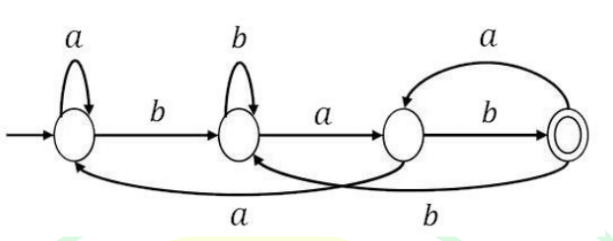
\includegraphics[width=0.5\columnwidth]{figs/q50.png}
        \caption*{}
        \label{fig:q50}
    \end{figure}

    Which of the following statements is/are FALSE?
    
    \begin{enumerate}
        \item States 2 and 4 are distinguishable in M
        \item States 3 and 4 are distinguishable in M
        \item States 2 and 3 are indistinguishable in M
        \item Any string w such that $n_0(w) = n_1(w)$ is in $L(M)$
    \end{enumerate}
    \hfill{\brak{\text{GATE CS 2024}}}

    \item The chromatic number of a graph is the minimum number of colours used in a proper colouring of the graph. Let G be any graph with n vertices and chromatic number k. Which of the following statements is/are always TRUE?
    \begin{enumerate}
        \item G contains a complete subgraph with k vertices
        \item G contains an independent set of size at least $n/k$
        \item G contains at least $k(k-1)/2$ edges
        \item G contains a vertex of degree at least k
    \end{enumerate}
    \hfill{\brak{\text{GATE CS 2024}}}

    \item Consider the operators $\oplus$ and $\Box$ defined by $a \oplus b = a+2b$ and $a \Box b = ab$, for positive integers. Which of the following statements is/are TRUE?
    \begin{enumerate}
        \item The operator $\diamond$ is associative
        \item The operator $\Box$ is associative
        \item Operator $\diamond$ over the operator $\Box$ obeys the distributive law
        \item Operator $\Box$ over the operator $\diamond$ obeys the distributive law
    \end{enumerate}
    \hfill{\brak{\text{GATE CS 2024}}}

    \item Consider two set-associative cache memory architectures: WBC, which uses the write back policy, and WTC, which uses the write through policy. Both of them use the LRU \brak{\text{Least Recently Used}} block replacement policy. The cache memory is connected to the main memory. Which of the following statements is/are TRUE?
    \begin{enumerate}
        \item A read miss in WBC never evicts a dirty block
        \item A read miss in WTC never triggers a write back operation of a cache block to main memory
        \item A write hit in WBC can modify the value of the dirty bit of a cache block
        \item A write miss in WTC always writes the victim cache block to main memory before loading the missed block to the cache
    \end{enumerate}
    \hfill{\brak{\text{GATE CS 2024}}}

    \item Consider a 512 GB hard disk with 32 storage surfaces. There are 4096 sectors per track and each sector holds 1024 bytes of data. The number of cylinders in the hard disk is \underline{\hspace{2cm}}.
    \item The baseline execution time of a program on a 2 GHz single core machine is 100 nanoseconds \brak{ns}. The code corresponding to 90\% of the execution time can be fully parallelized. The overhead for using an additional core is 10 ns when running on a multicore system. Assume that all cores in the multicore system run their share of the parallelized code for an equal amount of time.    
    The number of cores that minimize the execution time of the program is \underline{\hspace{2cm}}.
    \hfill{\brak{\text{GATE CS 2024}}}

    \item A given program has 25\% load/store instructions. Suppose the ideal CPI \brak{\text{cycles per instruction}} without any memory stalls is 2. The program exhibits 2\% miss rate on instruction cache and 8\% miss rate on data cache. The miss penalty is 100 cycles. The speedup \brak{\text{rounded off to two decimal places}} achieved with a perfect cache (i.e., with NO data or instruction cache misses) is \underline{\hspace{2cm}}.

    \hfill{\brak{\text{GATE CS 2024}}}

    \item Consider the following code snippet using the fork() and wait() system calls. Assume that the code compiles and runs correctly, and that the system calls run successfully without any errors.
    \begin{lstlisting}[language=C]
int x = 3;
while (x > 0) {
    fork();
    printf("hello");
    wait(NULL);
    x--;
}
    \end{lstlisting}
    The total number of times the printf statement is executed is \underline{\hspace{2cm}}.

    \hfill{\brak{\text{GATE CS 2024}}}

    \item Consider the entries shown below in the forwarding table of an IP router. Each entry consists of an IP prefix and the corresponding next hop router for packets whose destination IP address matches the prefix. The notation "/N" in a prefix indicates a subnet mask with the most significant N bits set to 1.
    
    \begin{table}[H]
        \centering
        \begin{tabular}{|l|l|}
        \hline
        \textbf{Prefix} & \textbf{Next hop router} \\
        \hline
        10.1.1.0/24 & R1 \\
        \hline
        10.1.1.128/25 & R2 \\
        \hline
        10.1.1.64/26 & R3 \\
        \hline
        10.1.1.192/26 & R4 \\
        \hline
        \end{tabular}
        \caption*{}
        \label{tab:q58}
    \end{table}
    
    This router forwards 20 packets each to 5 hosts. The IP addresses of the hosts are 10.1.1.16, 10.1.1.72, 10.1.1.132, 10.1.1.191, and 10.1.1.205. The number of packets forwarded via the next hop router R2 is \underline{\hspace{2cm}}.

    \hfill{\brak{\text{GATE CS 2024}}}

    \item Let $G=(V, \Sigma, S, P)$ be a context-free grammar in Chomsky Normal Form with $\Sigma=\{a,b,c\}$ and V containing 10 variable symbols including the start symbol S. The string $w=a^{30}b^{30}c^{30}$ is derivable from S. The number of steps \brak{application of rules} in the derivation $S \rightarrow^* w$ is \underline{\hspace{2cm}}.
    
    \hfill{\brak{\text{GATE CS 2024}}}

    \item The number of edges present in the forest generated by the DFS traversal of an undirected graph G with 100 vertices is 40. The number of connected components in G is \underline{\hspace{2cm}}.
    
    \hfill{\brak{\text{GATE CS 2024}}}

    \item Consider the following two regular expressions over the alphabet \{0,1\}:
    \begin{center}
    $r = 0^* + 1^*$
    
    $s = 01^* + 10^*$
    \end{center}
    
    
    The total number of strings of length less than or equal to 5, which are neither in r nor in s, is \underline{\hspace{2cm}}.

    \hfill{\brak{\text{GATE CS 2024}}}

    \item Consider a memory management system that uses a page size of 2 KB. Assume that both the physical and virtual addresses start from 0. Assume that the pages 0, 1, 2, and 3 are stored in the page frames 1, 3, 2, and 0, respectively. The physical address \brak{in decimal format} corresponding to the virtual address 2500 \brak{in decimal format} is \underline{\hspace{2cm}}.

    \hfill{\brak{\text{GATE CS 2024}}}

    \item A bag contains 10 red balls and 15 blue balls. Two balls are drawn randomly without replacement. Given that the first ball drawn is red, the probability \brak{rounded off to 3 decimal places} that both balls drawn are red is \underline{\hspace{2cm}}.

    \hfill{\brak{\text{GATE CS 2024}}}

    \item Consider a digital logic circuit consisting of three 2-to-1 multiplexers M1, M2, and M3 as shown below. X1 and X2 are inputs of M1. X3 and X4 are inputs of M2. A, B, and C are select lines of M1, M2, and M3, respectively.
    
    \begin{figure}[H]
        \centering
        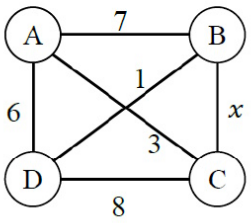
\includegraphics[width=0.3\columnwidth]{figs/q64.png}
        \caption*{}
        \label{fig:q64}
    \end{figure}
    
    For an instance of inputs $X1=1, X2=1, X3=0$ and $X4=0$, the number of combinations of A, B, C that give the output $Y=1$ is \underline{\hspace{2cm}}.

    \hfill{\brak{\text{GATE CS 2024}}}

    \item Consider sending an IP datagram of size 1420 bytes \brak{including 20 bytes of IP header} from a sender to a receiver over a path of two links with a router between them. The first link \brak{sender to router} has an MTU \brak{Maximum Transmission Unit} size of 542 bytes, while the second link \brak{router to receiver} has an MTU size of 360 bytes. The number of fragments that would be delivered at the receiver is \underline{\hspace{2cm}}.

    \hfill{\brak{\text{GATE CS 2024}}}

\end{enumerate}
\end{document}
